% !TEX root = ../../main.tex

\subsection{Specific surface area and pore volume calculations}

As adsorption takes place on the surface,
isotherms measured on porous materials are uniquely suited
for the determination of the accessible area of the void
space present inside the material structure or external
area of fine powders. \texttt{pyGAPS} comes with several
common methods used to
determine surface area, some with theoretical basis like
the IUPAC-recommended BET method and some empirical, such
as the t-plot method.

\subsubsection{BET surface area}\label{pyg:charac:betarea}

The BET method~\cite{brunauerAdsorptionGasesMultimolecular1938}
for determining surface area is the recommended IUPAC method~\cite{thommesPhysisorptionGasesSpecial2015}
to calculate the surface area of a porous material.
It is generally applied on isotherms obtained through \ce{N2}
adsorption at \SI{77}{\kelvin}, although other adsorbates
(\ce{Ar} at \SI{77}{\kelvin} or \SI{87}{\kelvin},
\ce{Kr} at \SI{77}{\kelvin}, \ce{CO2} at \SI{293}{\kelvin})
have been used. In principle, any probe with an adsorption behaviour
which can be described through the BET equation in the low pressure regime
can be used.

As previously mentioned, the method assumes that adsorption takes place
in incremental layers according to the
BET model (\ref{pyg:models:bet}).
Even if the adsorbent is porous, the initial amount adsorbed
(usually between 0.05--0.4 \(p/p_0\)) can be
described through the equation written in its linear form:

\begin{equation}
	\frac{p/p_0}{n_{ads} (1-p/p_0)} = \frac{1}{n_{m} C} + \frac{C - 1}{n_{m} C}(p/p_0)
\end{equation}

If we plot the isotherm points as
\({(p/p_0)}/{n_{ads}(1-p/p_0)}\) versus \(p/p_0\), a linear region
can usually be found. The slope and intercept of this line
can then be used to calculate \(n_{m}\), the amount adsorbed at the
statistical monolayer, as well as \(C\), the BET constant.

\begin{align}
	n_{m} & = \frac{1}{s+i} & C & = \frac{s}{i} + 1
\end{align}

From the BET monolayer capacity, the specific surface area can be
calculated if the area taken up by one of the adsorbate molecules
on the surface is known. The calculation uses the following equation
together with Avogadro's number:

\begin{equation}
	a_{BET} = n_m A_N \sigma
\end{equation}

While commonly used for surface area determination, the BET area
should be used with care, as the assumptions made in
its calculation may not hold. To augment the validity of the BET
method, Rouquerol~\cite{rouquerolAdsorptionPowdersPorous2013} proposed
several checks to ensure that the selected BET region is valid:

\begin{itemize}

	\item The BET (\(C\)) obtained should be positive;
	\item In the corresponding Rouquerol plot where \(n_{ads}(1-p/p_0)\)
	      is plotted with respect to \(p/p_0\), the points chosen for BET
	      analysis should be strictly increasing;
	\item The loading at the statistical monolayer should be
	      situated within the limits of the BET region.

\end{itemize}

All these checks are implemented in \texttt{pyGAPS}.
Regardless, the BET surface area should still be interpreted carefully.
Since adsorption takes place on the pore surface, microporous materials
which have pores of similar or smaller size as the probe molecule used
will not give a realistic surface area since in the micropore range
it is difficult to separate pore condensation behaviour from
multilayer adsorption. Furthermore, the cross-sectional
area of the molecule on the surface cannot be guaranteed. For example,
nitrogen has been known to adopt a different conformation on the surface
of some materials due to inter-molecular forces, which effectively
lowers its cross-sectional area~\cite{rouquerolAdsorptionPowdersPorous2013}.

In \texttt{pyGAPS}, starting from an isotherm object, it is easy to
calculate the BET area by using the code in Listing~\ref{pyg:lst:betarea}.
The framework automatically applies the Rouquerol rules to
find the optimum pressure range and returns the results as a
dictionary. The \inline{verbose=True} option prints a short
text with all the calculation variables as well as graphing the
BET and Rouquerol plots (Figure~\ref{pyg:fgr:betarea}).
The user can override
automatic pressure range selection by using the range parameter
(\inline{limits=(0.05, 0.3)}).

\begin{samepage}
	\begin{python}[caption={Calculating a BET area},label={pyg:lst:betarea}]
area_dict = pygaps.area_BET(isotherm, verbose=True)
\end{python}
	\begin{pythonout}
BET surface area: a = 1277 m2/g
Minimum pressure point chosen is 0.005 and maximum is 0.034
The slope of the BET fit: 		s = 76.344
The intercept of the BET fit: 	i = 0.052
BET constant: 					C = 1463
Amount for a monolayer: 		n = 0.01309 mol/g
\end{pythonout}
\end{samepage}

\begin{figure}[!htb]
	\centering

	\begin{subfigure}{0.45\linewidth}
		\parbox[c]{0.1\linewidth}{\caption{}%
			\label{pyg:fgr:betarea-plt}}
		\parbox[b]{0.85\linewidth}{%
			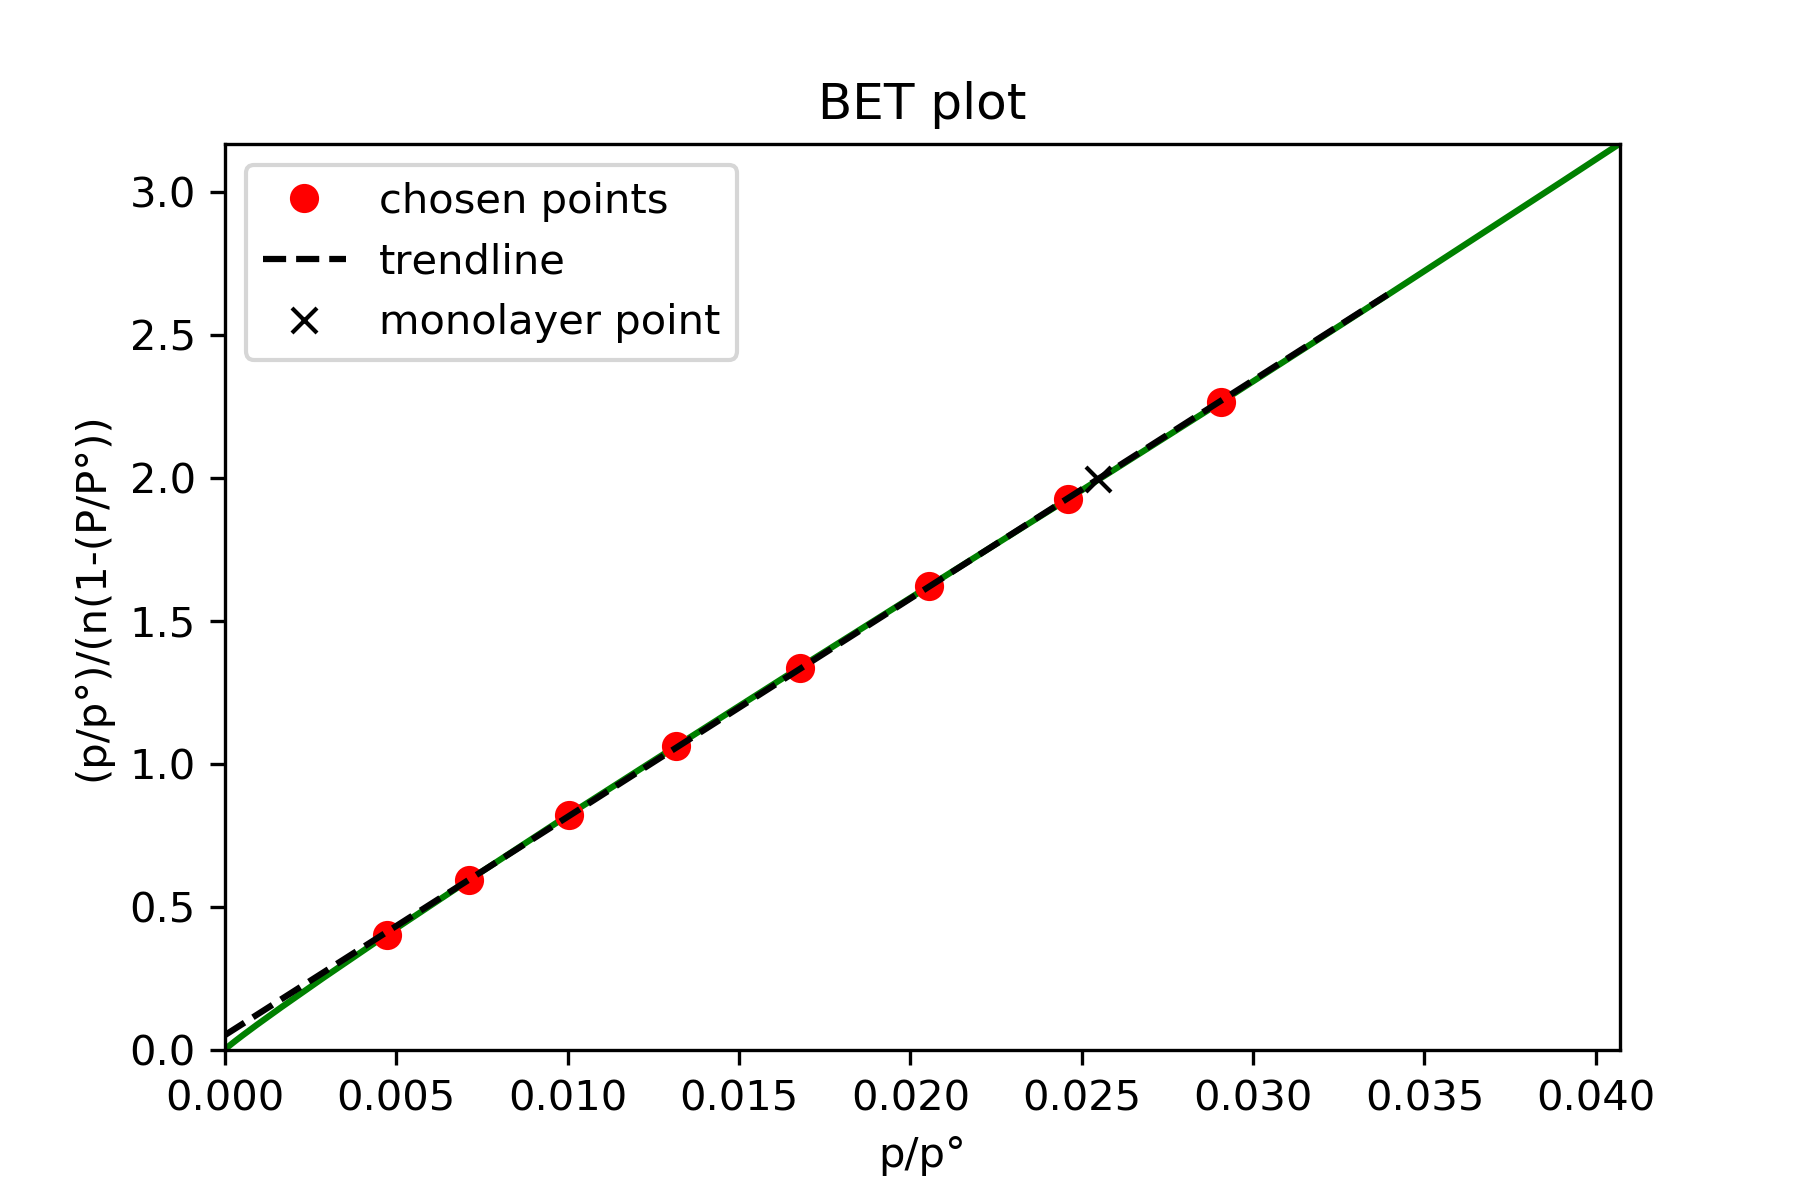
\includegraphics[width=\linewidth]{characterization/bet-plt}}
	\end{subfigure}
	\begin{subfigure}{0.45\linewidth}
		\parbox[c]{0.1\linewidth}{\caption{}%
			\label{pyg:fgr:betarea-roq}}
		\parbox[b]{0.85\linewidth}{%
			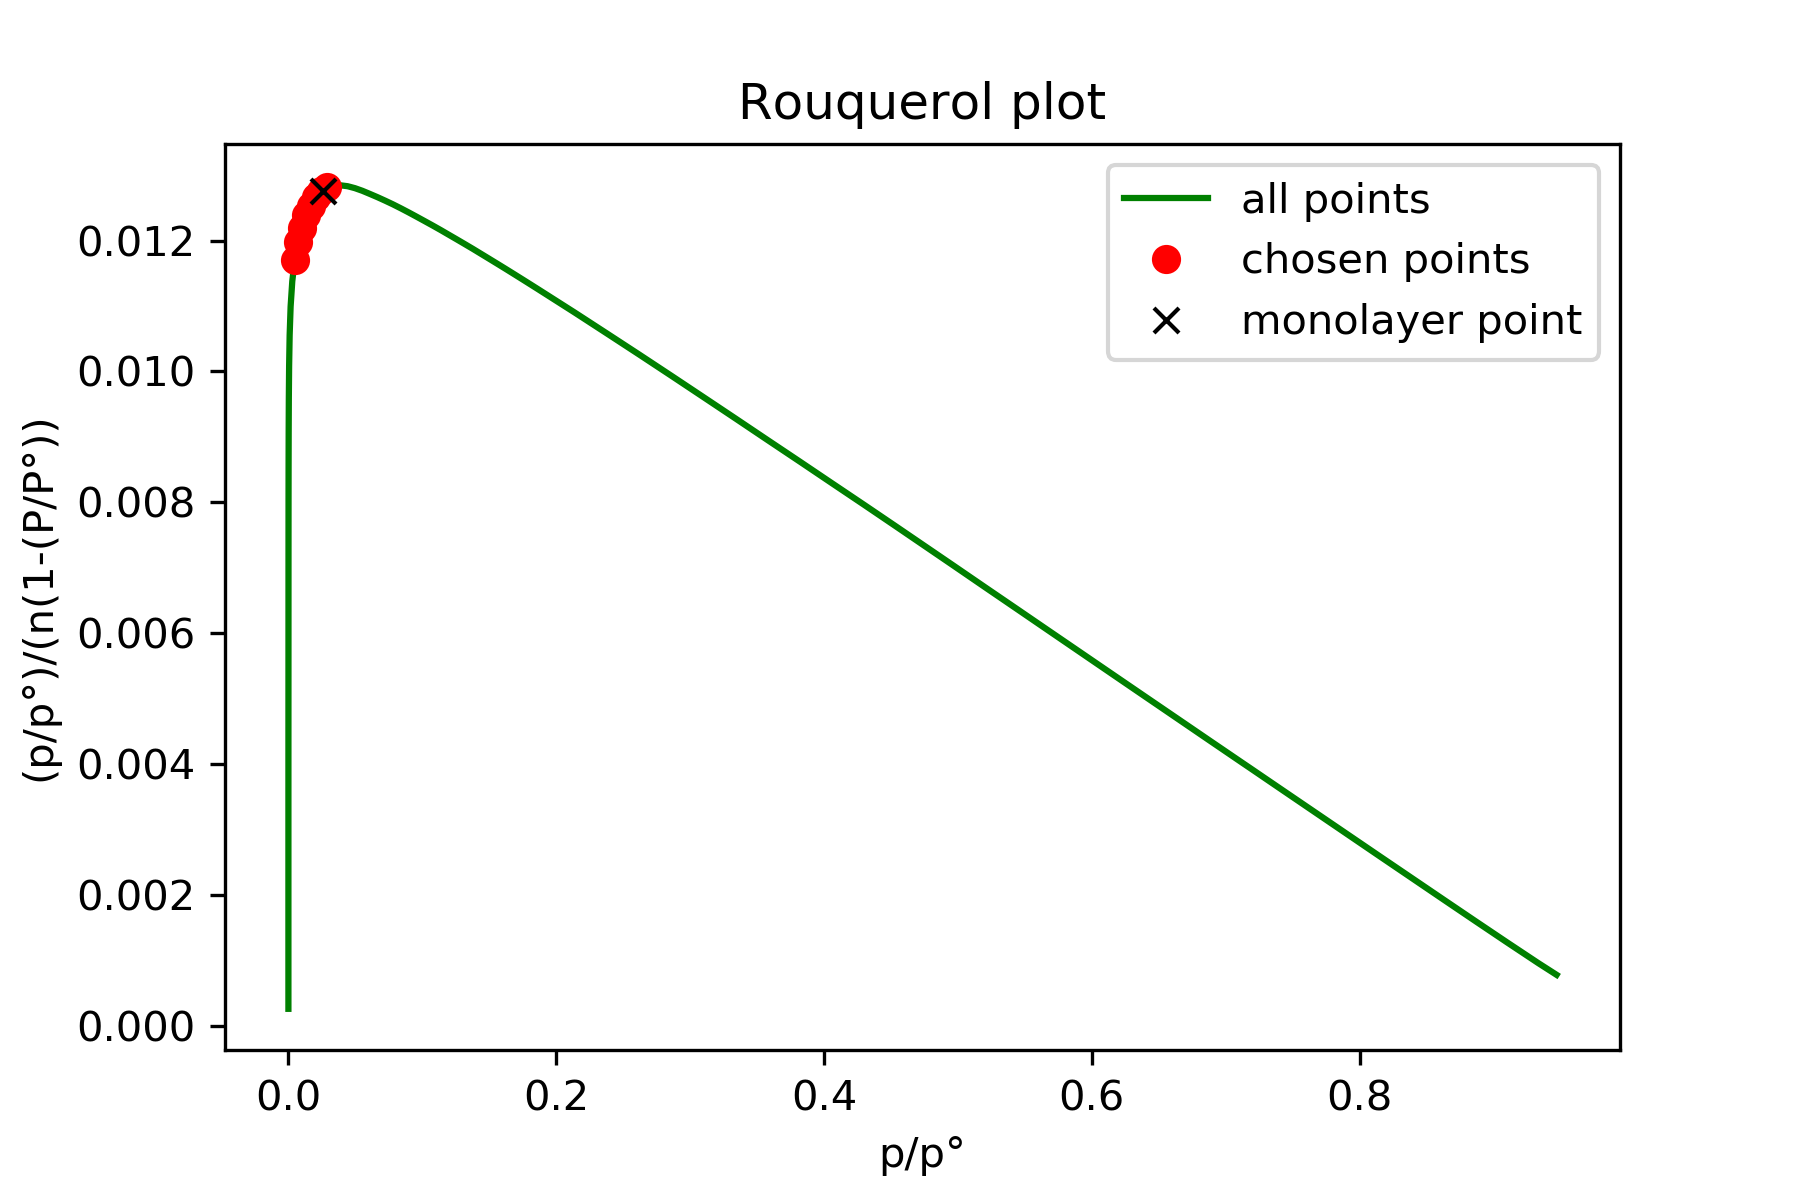
\includegraphics[width=\linewidth]{characterization/bet-roq}}
	\end{subfigure}

	\caption{Output from the BET area function (a) the BET plot showing
		the selected points for fitting the equation, as well as the location
		of the statistical monolayer and (b) the Rouquerol plot for this
		calculation.}%
	\label{pyg:fgr:betarea}

\end{figure}

\subsubsection{Langmuir surface area}\label{pyg:charac:langmuirarea}

The Langmuir equation (\ref{pyg:eqn:langmuir}) can be also
be expressed in a linear form by rearranging it as:

\begin{equation}
	\frac{p}{n} = \frac{1}{K n_m} + \frac{p}{n_m}
\end{equation}

Assuming the data can be fitted with a Langmuir model, by plotting
\({p}/{n}\) against pressure, a straight line will be obtained. The slope and
intercept of this line can then be used to calculate \(n_{m}\),
the amount adsorbed at the monolayer, as well as \(K\), the Langmuir constant.

\begin{align}
	n_m & = \frac{1}{s} & K & = \frac{1}{i * n_m}
\end{align}

The surface area can then be calculated by using the monolayer
capacity in a manner analogous to the BET surface area method.

\begin{equation}
	a_{Langmuir} = n_m A_N \sigma
\end{equation}

The Langmuir method for determining surface area assumes that
adsorption takes place until all active sites on the material
surface are occupied, or until monolayer formation in the
case of complete surface coverage. As most adsorption processes
(except chemisorption) don't follow this behaviour, it is
important to regard the Langmuir surface area as an estimate.

As with the BET area, the Langmuir area is calculated by using the code in
Listing~\ref{pyg:lst:langmuirarea}. The framework will alert the user
if the correlation is not linear in the selected range.
Here the \inline{verbose=True} option prints a short
text with all the calculation variables and the graphs the
Langmuir plot as seen in Figure~\ref{pyg:fgr:langmuirarea-auto}.
If desired the user can override
automatic pressure range selection as seen in the second example in
Listing~\ref{pyg:lst:langmuirarea}.

\begin{samepage}
	\begin{python}[caption={Calculating a Langmuir area},label={pyg:lst:langmuirarea}]
area_dict = pygaps.area_langmuir(isotherm, verbose=True)
\end{python}
	\begin{pythonout}
WARINING The correlation is not linear!
\end{pythonout}
	\begin{python}
area_dict = pygaps.area_langmuir(isotherm, 
                                 limits=(0.05, 0.3), 
                                 verbose=True)
\end{python}
	\begin{pythonout}
Langmuir surface area: 	a = 415 m2/g
Minimum pressure point chosen is 0.0 and maximum is 0.194
The slope of the Langmuir line: 		s = 234.968
The intercept of the Langmuir line: 	i = 1.607
The Langmuir constant is:				K = 146
Amount for a monolayer: 				n = 0.00426 mol/g
\end{pythonout}
\end{samepage}

\begin{figure}[!htb]
	\centering

	\begin{subfigure}{0.45\linewidth}
		\parbox[c]{0.1\linewidth}{\caption{}%
			\label{pyg:fgr:langmuirarea-auto}}
		\parbox[b]{0.85\linewidth}{%
			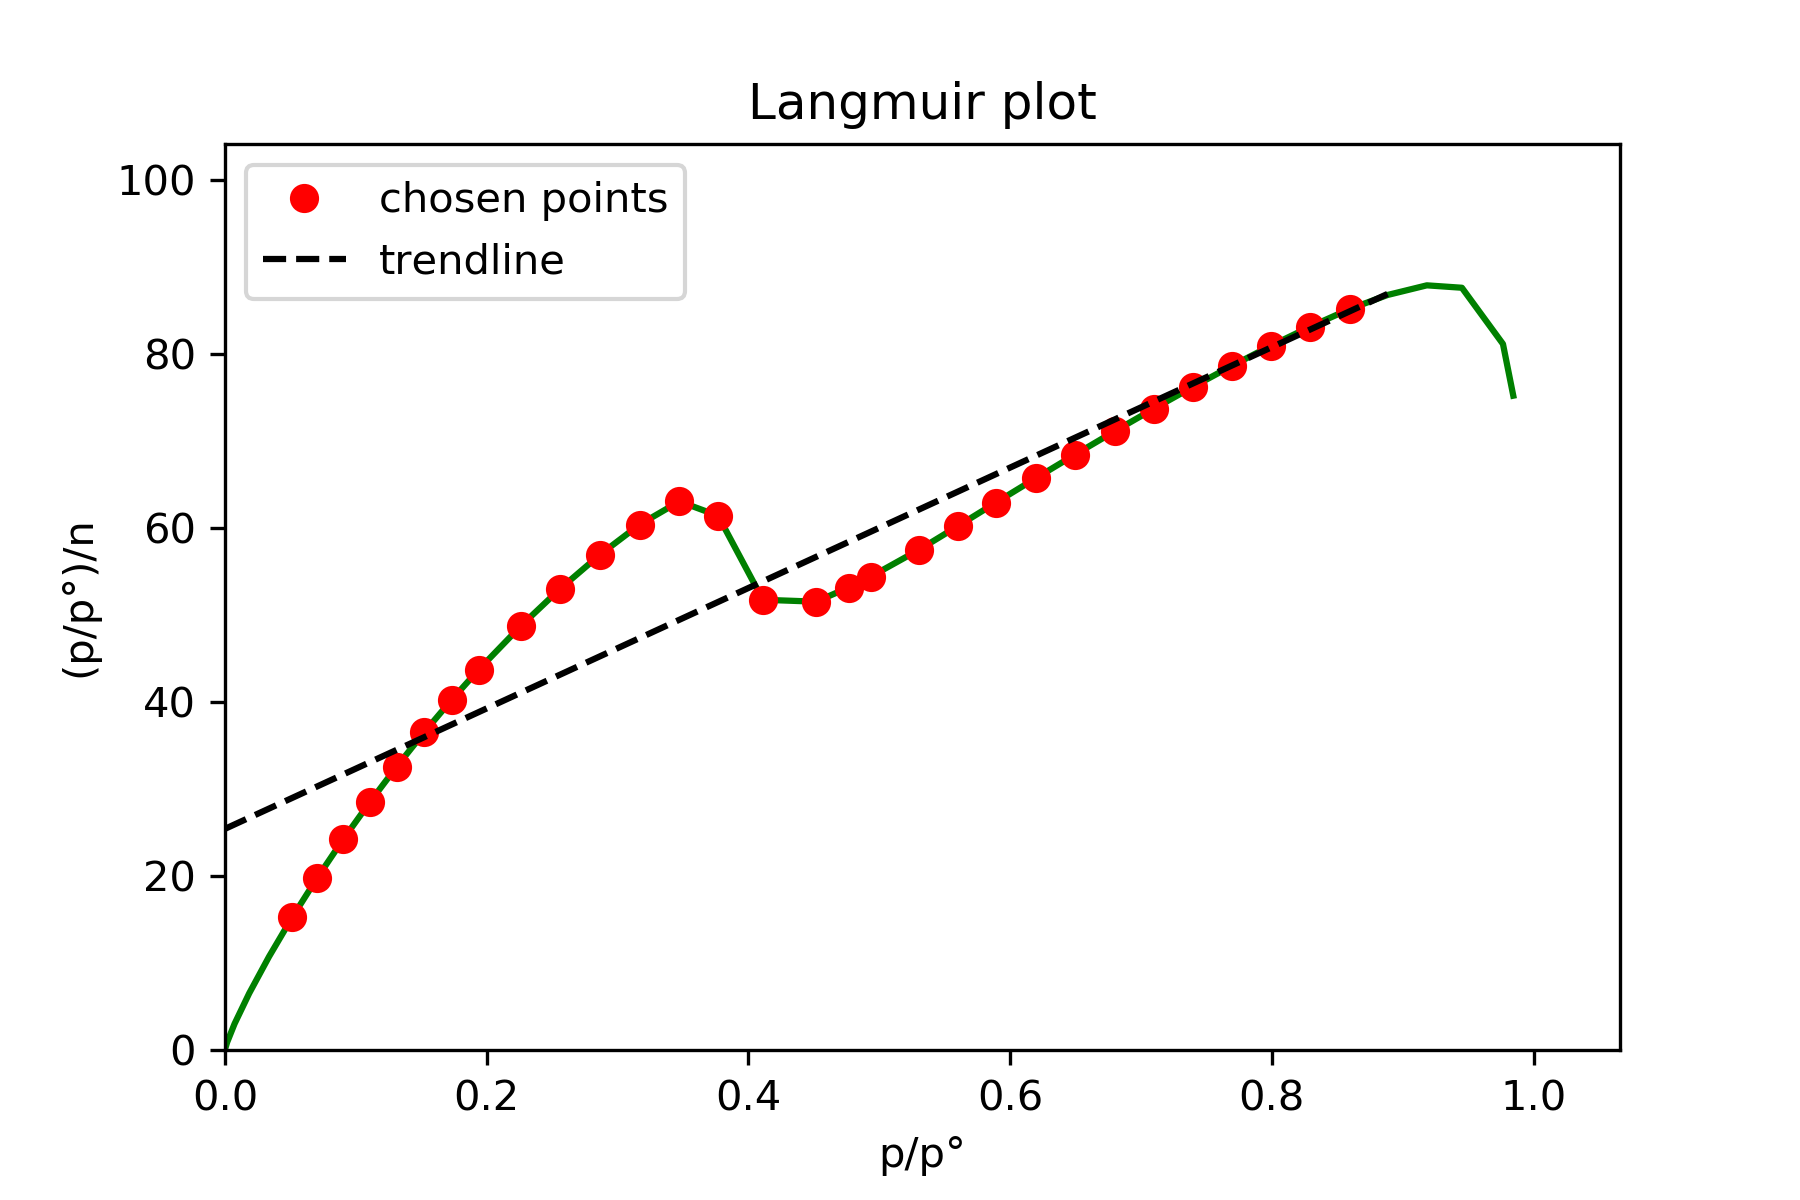
\includegraphics[width=\linewidth]{characterization/langmuir-auto}}
	\end{subfigure}
	\begin{subfigure}{0.45\linewidth}
		\parbox[c]{0.1\linewidth}{\caption{}%
			\label{pyg:fgr:langmuirarea-manual}}
		\parbox[b]{0.85\linewidth}{%
			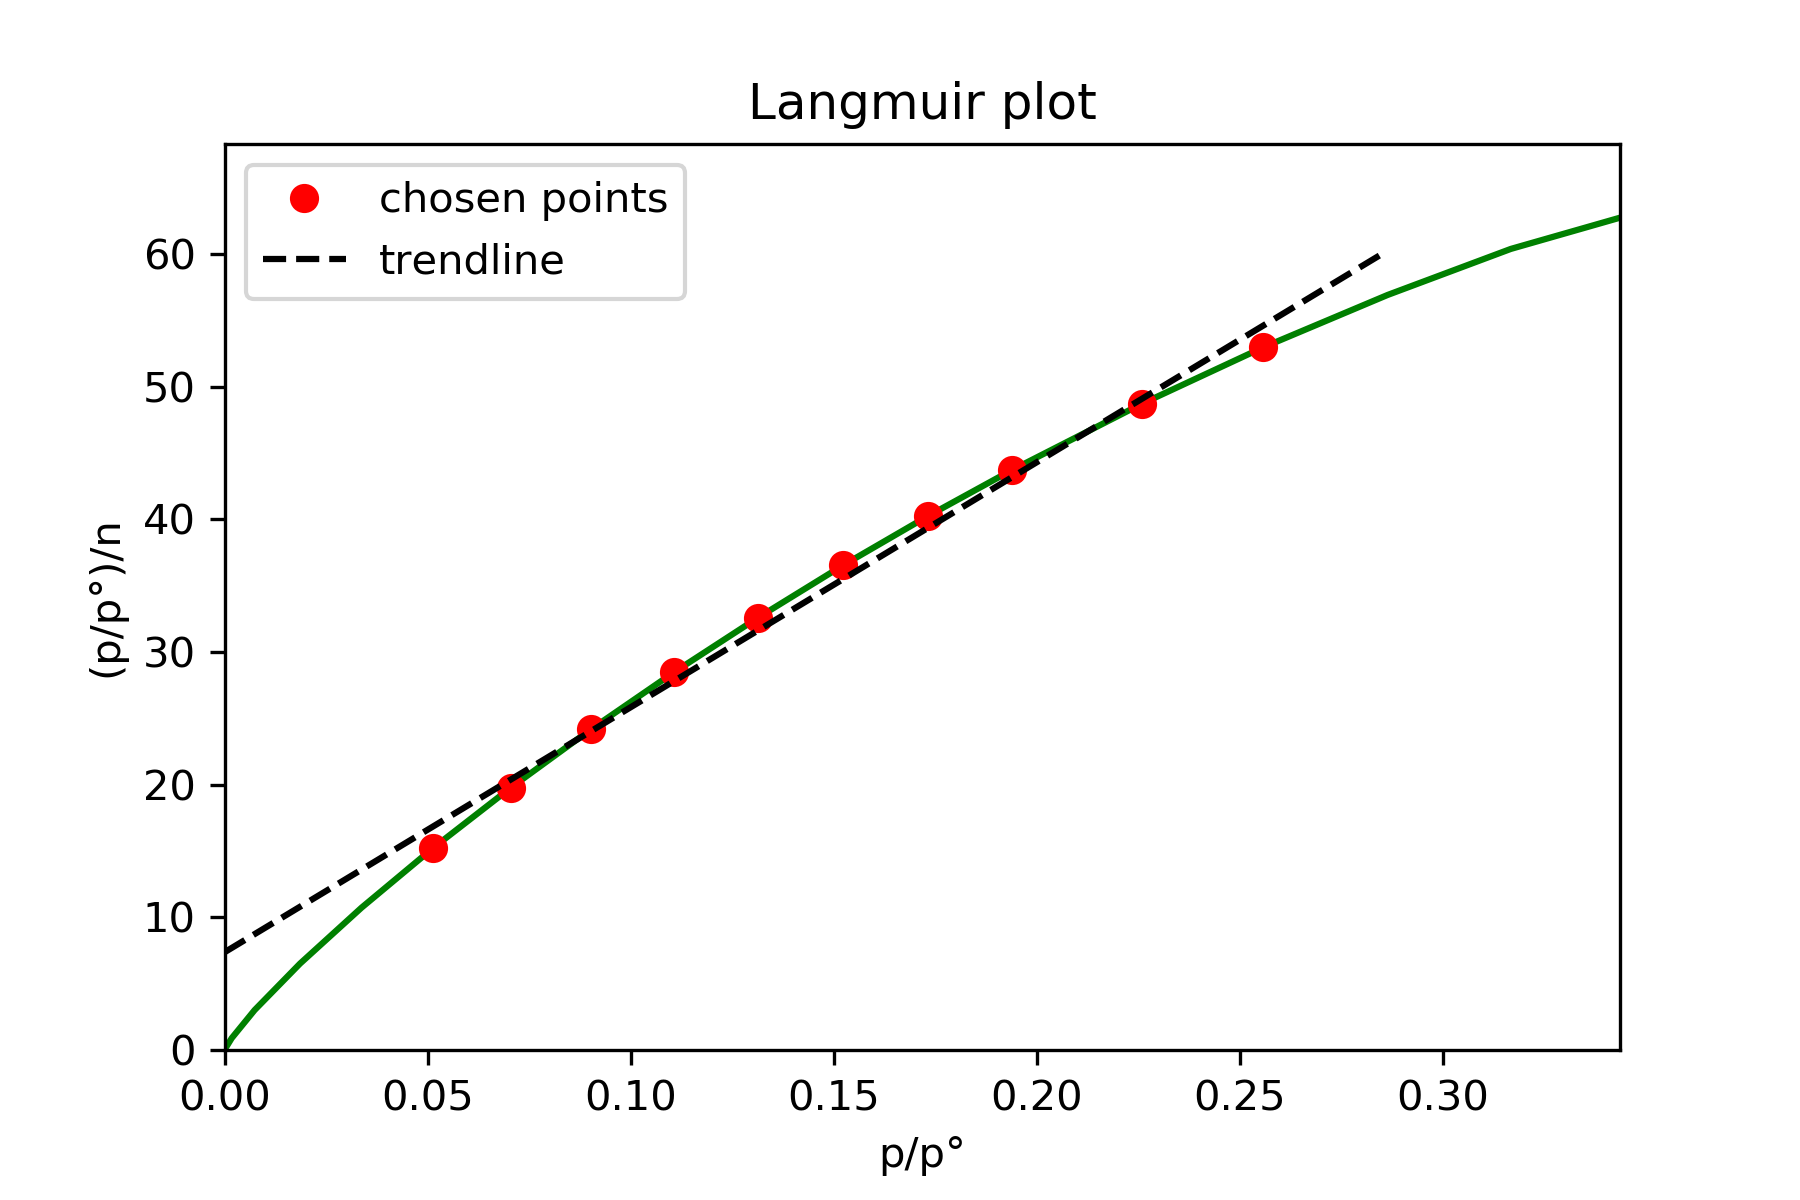
\includegraphics[width=\linewidth]{characterization/langmuir-manual}}
	\end{subfigure}

	\caption{Output from the Langmuir area function (a) the Langmuir plot
		showing the automatic fitting attempt which generates a warning and (b) a manually
		selected pressure range for the Langmuir plot.}%
	\label{pyg:fgr:langmuirarea}

\end{figure}

\subsubsection{Ideal isotherms or thickness functions}\label{pyg:charac:tcurve}

The initial part of an isotherm (the Henry regime) can be seen to
be very dependent on the interactions between the adsorbate and the
surface. However, the subsequent layers are less influenced by the
material and can often be assumed, like in the BET model,
to have an energy of adsorption identical to the enthalpy of liquefaction
of the bulk liquid and therefore, their formation depends essentially
only on the partial pressure.

With this assumption, several studies have been focused on obtaining
an ``ideal'' isotherm of adsorption on a non-porous material which can
then, if the cross-sectional area of the molecule is known, be transformed
in a function capable of predicting the multilayer thickness
as a function of pressure. This kind of empirical function,
also referred to as a \textit{thickness function} or \textit{t-curve},
can then be used as an
alternative method for surface area determination, as explained in
the next section. These curves are also used in the classical methods
for calculating mesoporous size distributions. It is important to
clarify that the function is only applicable for a single adsorbent
and a single temperature.

Several common thickness functions have been implemented in \texttt{pyGAPS},
applicable for nitrogen at \SI{77}{\kelvin}
such as the Halsey~\cite{halseyPhysicalAdsorptionNon1948}
(equation~\ref{pyg:eqn:halsey}) and the
Harkins and Jura~\cite{harkinsSurfacesSolidsXIII1944a}
(equation~\ref{pyg:eqn:harkinsjura}) curve.

\todo{check equations}
\begin{align}
	t_{Halsey}        & = 0.354 {\Big(\frac{-5}{\log(p/p_0)}\Big)}^{1/3} \label{pyg:eqn:halsey}                 \\
	t_{Harkins\&Jura} & = {\Big(\frac{0.1399}{0.034 - \log_{10}(p/p_0)}\Big)}^{1/2} \label{pyg:eqn:harkinsjura}
\end{align}

These t-curves are selected by name as parameters in
the functions that use them. The user can also define their
own t-curve as a function and pass it as a parameter. An example
is shown in Listing~\ref{pyg:lst:tplot} in the t-plot section.

\subsubsection{t-plot Method}\label{pyg:charac:tplot}

The t-plot method is an empirical method, developed as a
tool to determine the surface area of porous materials,
which can also be used for other calculations, such as
external pore area and micropore volume
calculations~\cite{lippensStudiesPoreSystems1965}.
A plot is constructed, where the isotherm loading
data is plotted versus the ideal thickness of the adsorbate layer,
obtained through the a t-curve (Section~\ref{pyg:charac:tcurve}).
It stands to reason that, in the case when the experimentally measured
loading follows the model, a straight line will be obtained with its
intercept through the origin. However, since in most cases there
are differences between adsorption in the pores and ideal surface
adsorption, the t-plot will deviate and form features which can
be analysed to describe the material characteristics.

\begin{itemize}

	\item A sharp vertical deviation will indicate condensation
	      in a type of mesopore structure.
	\item A gradual slope will indicate adsorption on a specific
	      surface.

\end{itemize}

The slope of the linear section can be used to calculate the area where
adsorption is taking place. If the linear region occurs at low loadings,
it will represent the total surface area of the material.
If at the end of the curve, it will instead represent adsorption on
the external surface area of the sample. The formula to calculate the area
is presented in Equation~\ref{pyg:fgr:areatplot},
where \(\rho_{l}\) is the liquid density of the adsorbate at experimental
conditions.

\begin{equation}\label{pyg:fgr:areatplot}
	a_{surface} = \frac{s M_m}{\rho_{l}}
\end{equation}

If the region selected is after a vertical deviation, the intercept of 
the line will no longer pass through the origin. This intercept can 
be used to calculate the volume of the filled pore through the 
following equation:

\begin{equation}
	V_{ads} = \frac{i M_m}{\rho_{l}}
\end{equation}

Since the t-plot method is comparing the experimental isotherm 
with an ideal model, care must be taken to ensure that the t-curve
is an accurate representation of the thickness of the 
adsorbate multilayers on the surface of the adsorbent. 
Since there is no such thing as a universal thickness curve,
care must be taken when selecting a thickness model to ensure that it
is applicable to both the material and the adsorbate.
Also, features on the t-plot found at loadings lower than the monolayer
thickness do not have any physical meaning.

In \texttt{pyGAPS}, when the function is called without any parameters
except an isotherm, the framework will attempt to find 
plateaus in the data and
automatically fit them with a straight line, returning a dictionary
with the slope, intercept and calculated pore volume and specific area
for each linear region found. As an example, the first function in
Listing~\ref{pyg:lst:tplot} will generate the graph in
Figure~\ref{pyg:fgr:tplot-auto}. The isotherm in this example is measured
on a sample of MCM-41.

\begin{python}[float=htb, caption={Generating a t-plot},%
    label={pyg:lst:tplot}]
# using automatic region detection
pygaps.t_plot(isotherm, verbose=True)

# specifying a manual region
pygaps.t_plot(isotherm, limits=(0.3,0.44), verbose=True)

# using the Halsey thickness curve
pygaps.t_plot(isotherm, thickness_model='Halsey', verbose=True)

# defining a custom t-curve to use in the t-plot
def carbon_model(relative_p):
	return 0.88*(relative_p**2) + 6.45*relative_p + 2.98

pygaps.t_plot(isotherm, thickness_model=carbon_model, verbose=True)
\end{python}

\begin{figure}[!htb]
	\centering

	\begin{subfigure}{0.45\linewidth}
		\parbox[c]{0.1\linewidth}{\caption{}%
			\label{pyg:fgr:tplot-auto}}
		\parbox[b]{0.85\linewidth}{%
			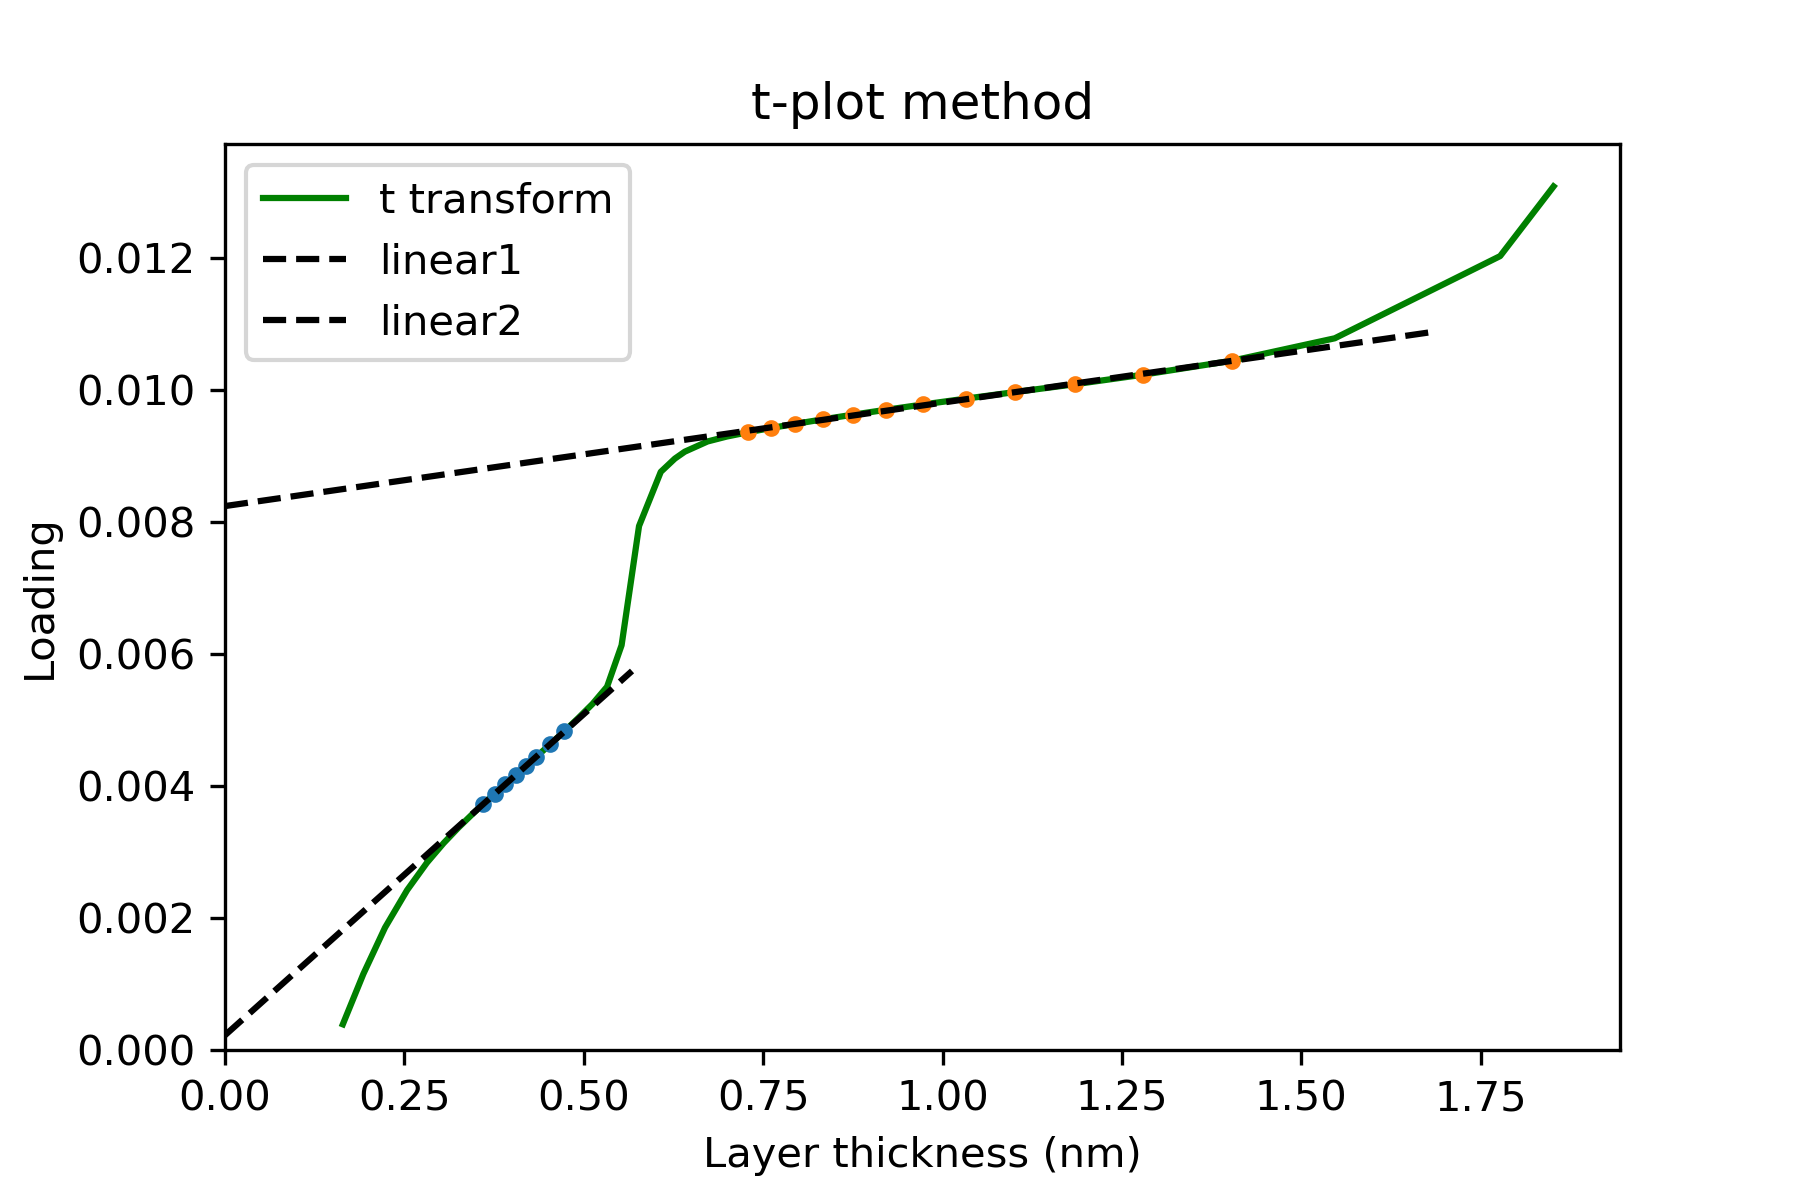
\includegraphics[width=\linewidth]{characterization/tplot-auto}}
	\end{subfigure}
	\begin{subfigure}{0.45\linewidth}
		\parbox[c]{0.1\linewidth}{\caption{}%
			\label{pyg:fgr:tplot-manual}}
		\parbox[b]{0.85\linewidth}{%
			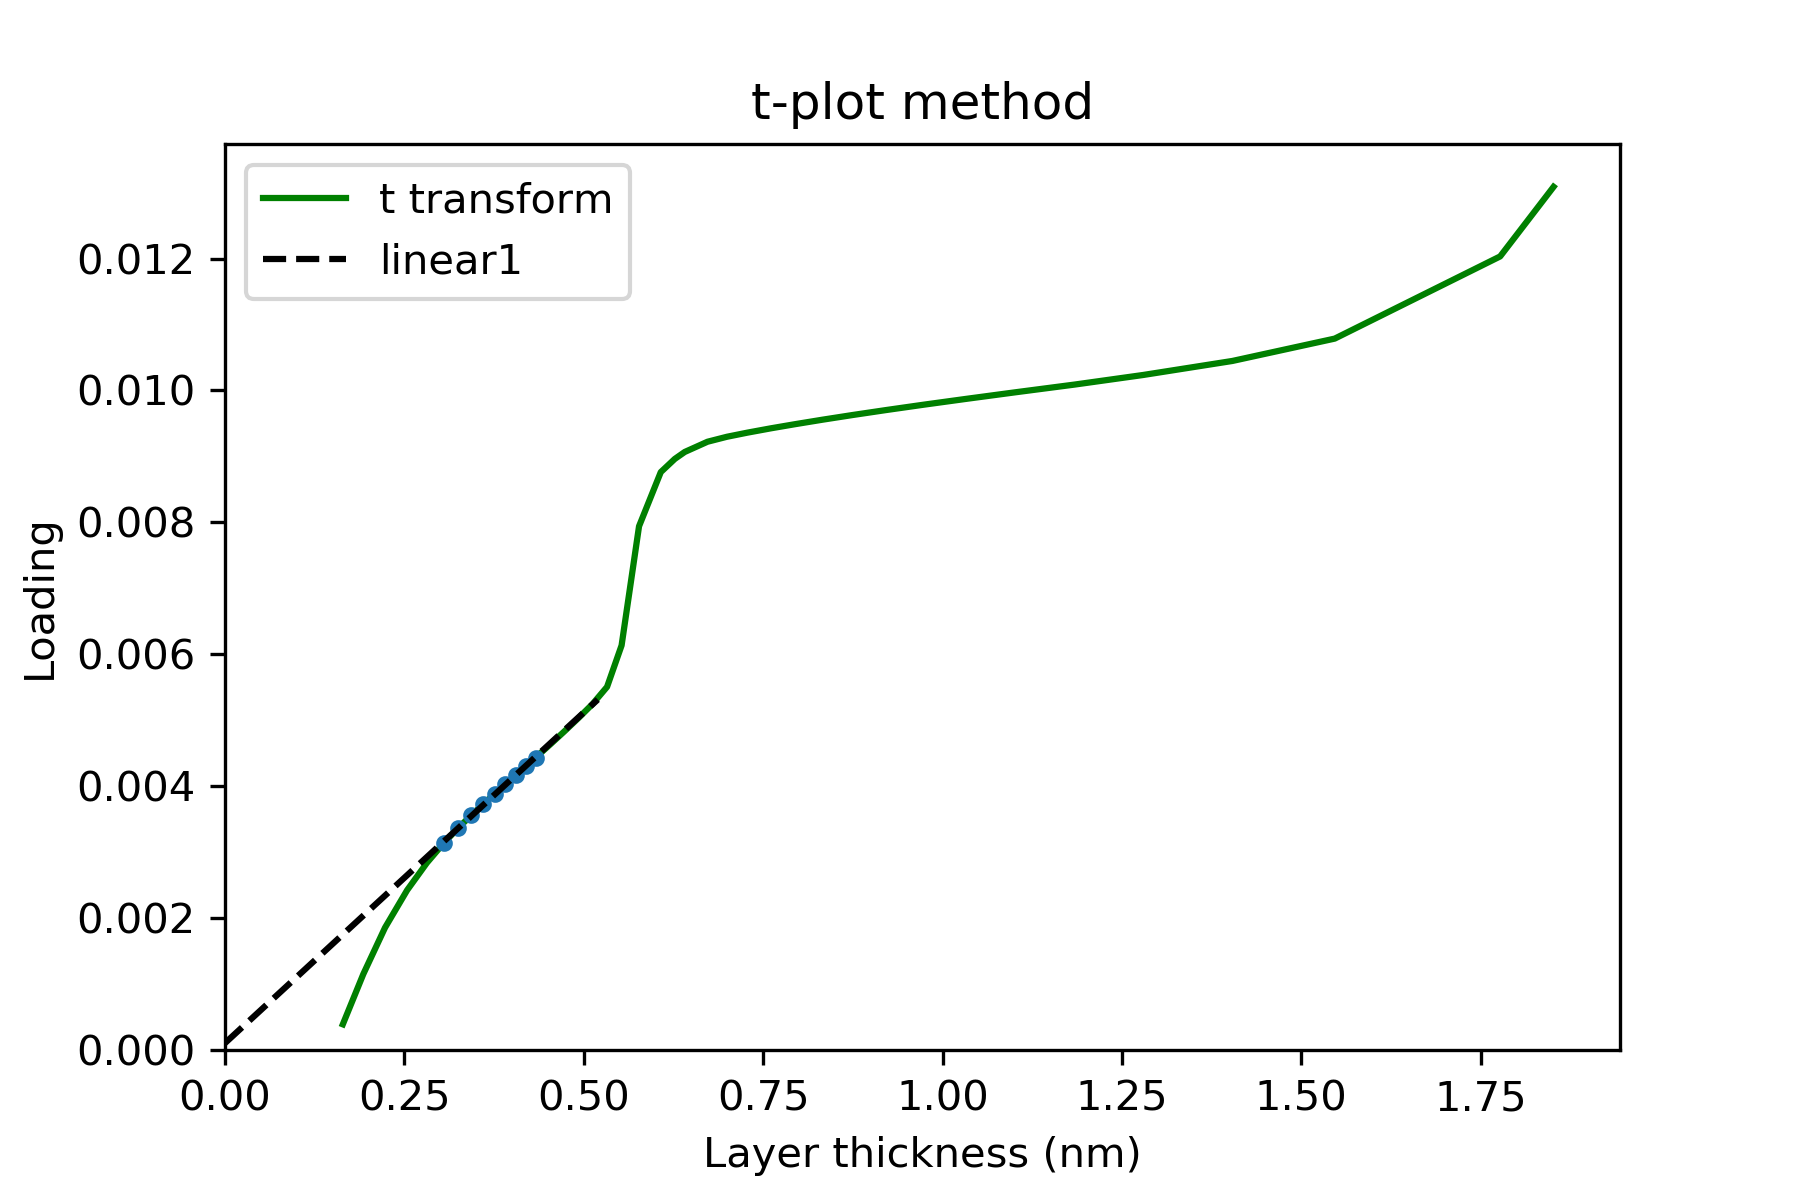
\includegraphics[width=\linewidth]{characterization/tplot-manual}}
	\end{subfigure}

	\caption{Output from the t-plot method function (a) an automatically
		obtained t-plot with the calculated fit regions and (b) a manually
		selected range for the t-plot.}%
	\label{pyg:fgr:tplot}

\end{figure}

The first linear region in Figure~\ref{pyg:fgr:tplot-auto} can be attributed
to adsorption on the mesopore surface,
while the second one represents adsorption on the available surface
after mesopore filling. Therefore, the surface area values calculated 
for the first and second region correspond to the area of the mesopores
and the external particle area, respectively. As only one pore filling 
event occurs, the pore volume calculated for the second region gives
us the mesopore volume. We can obtain a more accurate result for the
surface area by fitting the first linear region to a zero intercept
through manual region selection, as shown in the second example in 
Listing~\ref{pyg:lst:tplot}.

Finally, the framework allows for the thickness model to be substituted
with an user-provided function which will be used for the t-plot, 
as mentioned before in Section~\ref{pyg:charac:tcurve}.
Usage of a carbon black-type thickness curve is presented in the last
example in Listing~\ref{pyg:lst:tplot}.

\subsubsection{\(\alpha_s\) Method}\label{pyg:charac:alphasplot}

In order to extend the t-plot analysis with other adsorbents and 
non-standard thickness curves, the \(\alpha_s\) method was
devised~\cite{atkinsonAdsorptivePropertiesMicroporous1984}.
Instead of attempting to find an ideal isotherm that describes the
thickness of the adsorbed layer, a reference isotherm is used.
This isotherm is measured on a non-porous version of the same material,
assumed to have identical surface characteristics.
The dimensionless \(\alpha_s\) values are obtained from this isotherm by
dividing the loading values by the amount adsorbed at a specific relative
pressure, usually taken as \(p/p_0=0.4\) since nitrogen hysteresis loops
theoretically close at this point.

\begin{equation}
	\alpha_s = \frac{n_a}{n_{0.4}}
\end{equation}

The analysis then proceeds as in the t-plot method, with the 
same explanation for observed features. The only difference is
that the surface area calculation from linear regions observed
uses the known specific area of the reference material.

\begin{equation}
	A = \frac{s A_{ref}}{(n_{ref})_{0.4}}
\end{equation}

The reference isotherm chosen for the \(\alpha_s\) method must 
be a description of the adsorption on a completely non-porous sample
of the same material. It is often impossible to obtain such 
non-porous versions, therefore care must be
taken how the reference isotherm is measured.

To generate an \(\alpha_s\)-plot in \texttt{pyGAPS}, both 
an analysis isotherm and a reference isotherm must be supplied 
as shown in Listing~\ref{pyg:lst:alphasplot}.
In this example, the reference isotherm is measured on non-porous silica.
The reference material area can be specified by using 
the \inline{reference_area} parameter. If not specified, it 
is automatically calculated by applying the BET
method on the reference isotherm.

\begin{python}[caption={Generating an \(\alpha_s\)-plot},label={pyg:lst:alphasplot}]
pygaps.alpha_s(isotherm, 
			   reference_isotherm=isotherm_r,
			   verbose=True)
\end{python}

\begin{figure}[!htb]
	\centering

	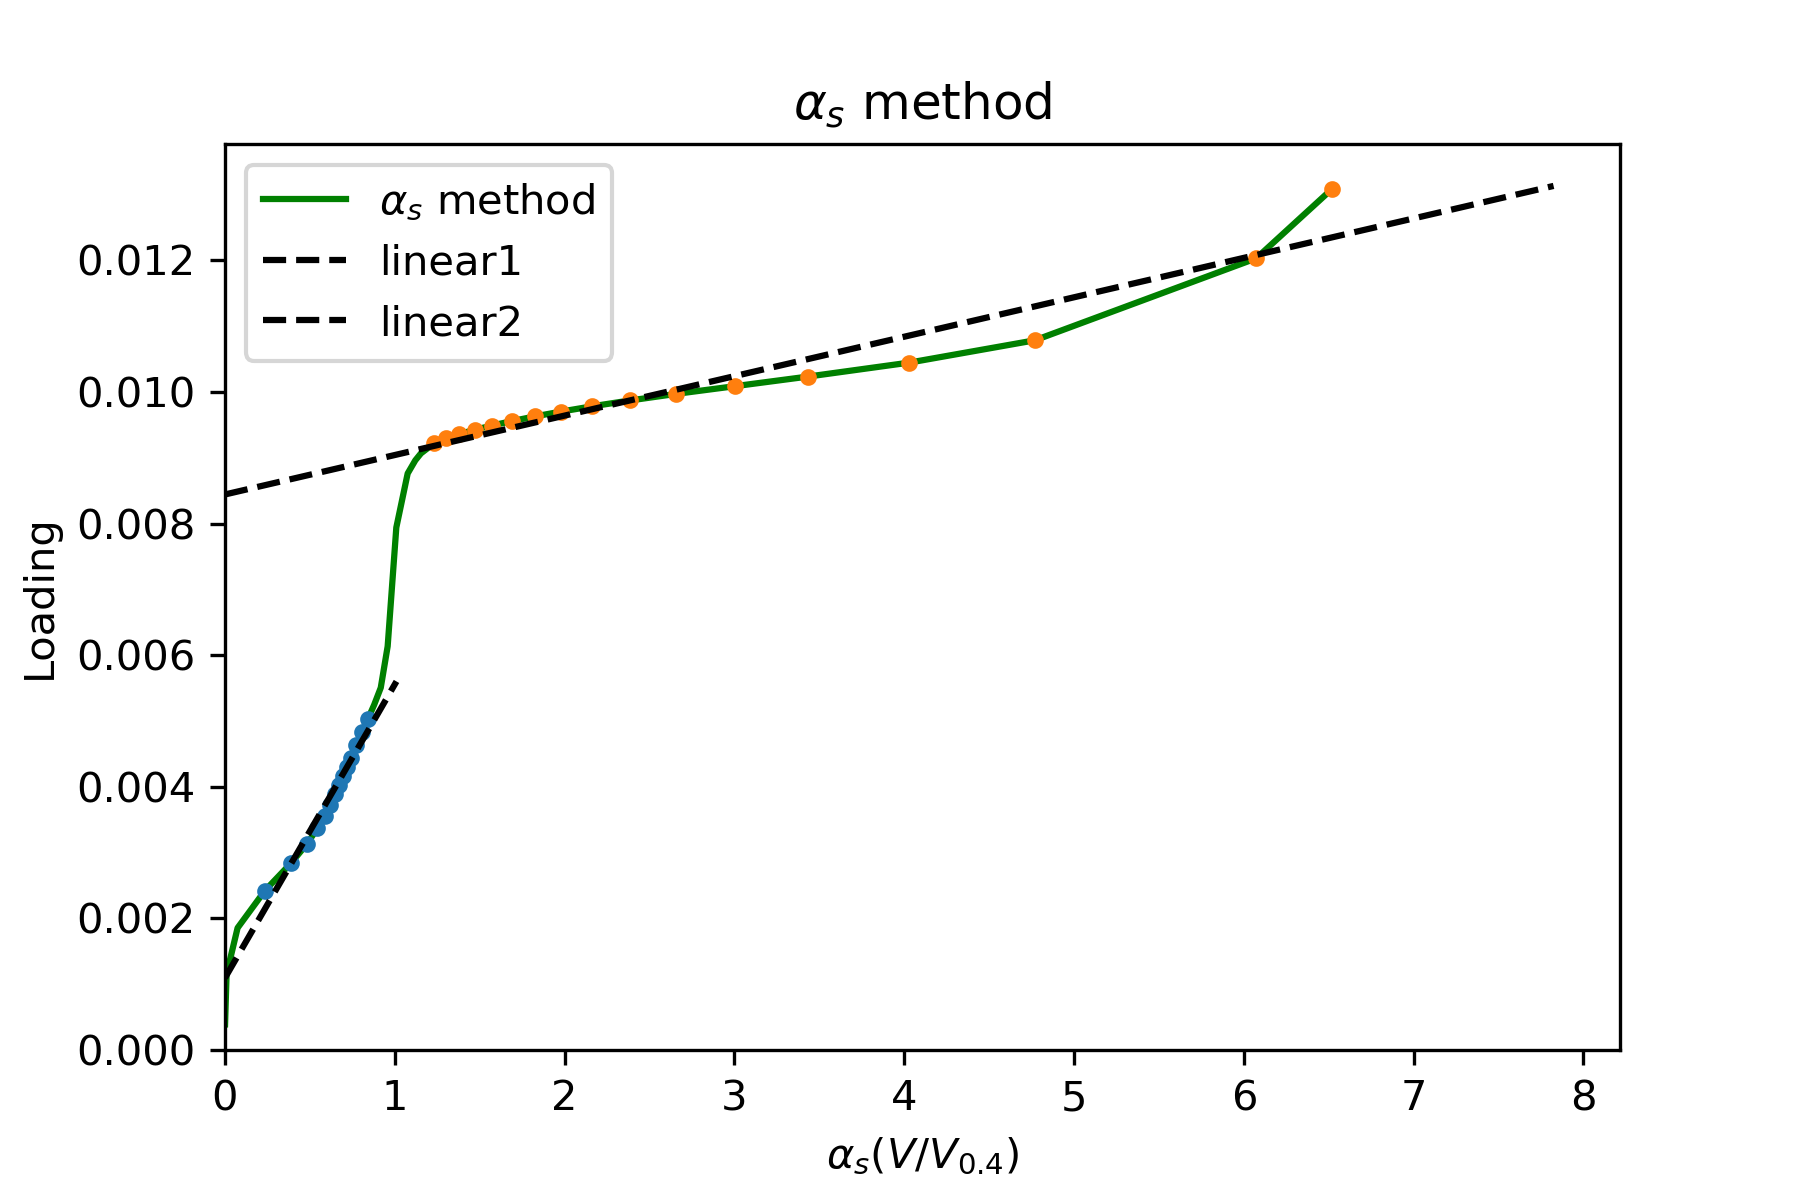
\includegraphics[width=0.45\linewidth]{characterization/alphas-auto}
	\caption{Output from the \(\alpha_s\)-plot function showing two
		automatically fit regions.}%
	\label{pyg:fgr:alphasplot}

\end{figure}
